%% fig_quarticloci.tex   (generated by make_round12.py; do not edit by hand)
%% Where the Weil classes of a quartic CM family are known to be algebraic.
\documentclass[tikz,border=8pt]{standalone}
\usepackage{amsmath,amssymb}
\usetikzlibrary{arrows.meta,calc,decorations.pathreplacing}
%% palette.tex -- shared colour definitions for the figures
\definecolor{PInk}{RGB}{26,32,44}
\definecolor{PBlue}{RGB}{37,82,139}
\definecolor{PTeal}{RGB}{23,127,125}
\definecolor{POchre}{RGB}{193,138,44}
\definecolor{PClay}{RGB}{178,74,58}
\definecolor{PSlate}{RGB}{108,122,137}
\definecolor{PViolet}{RGB}{110,86,150}
\definecolor{WBlue}{RGB}{223,234,246}
\definecolor{WTeal}{RGB}{220,238,236}
\definecolor{WOchre}{RGB}{250,240,218}
\definecolor{WClay}{RGB}{247,229,224}
\definecolor{WSlate}{RGB}{238,241,244}
\definecolor{PMag}{RGB}{158,58,110}
\definecolor{PGrass}{RGB}{62,124,66}
\definecolor{PAmber}{RGB}{214,112,38}
\definecolor{PIndigo}{RGB}{58,64,140}
\definecolor{PRule}{RGB}{176,186,197}

%% shared macros so the standalone figures match the paper
\providecommand{\QQ}{\mathbb{Q}}
\providecommand{\ZZ}{\mathbb{Z}}
\providecommand{\RR}{\mathbb{R}}
\providecommand{\CC}{\mathbb{C}}
\providecommand{\PP}{\mathbb{P}}
\providecommand{\Kx}{K^{\times}}
\providecommand{\HW}{W}
\providecommand{\Nm}{\mathrm{N}}
\providecommand{\Hdg}{\mathrm{Hdg}}
\providecommand{\NS}{\mathrm{NS}}
\providecommand{\cA}{\mathcal{A}}
\providecommand{\cD}{\mathcal{D}}
\providecommand{\cF}{\mathcal{F}}
\providecommand{\cP}{\mathcal{P}}
\providecommand{\cO}{\mathcal{O}}
\providecommand{\cQ}{\mathcal{Q}}
\providecommand{\bbar}[1]{\overline{#1}}
\providecommand{\ch}{\operatorname{ch}}
\providecommand{\End}{\mathrm{End}}

\begin{document}
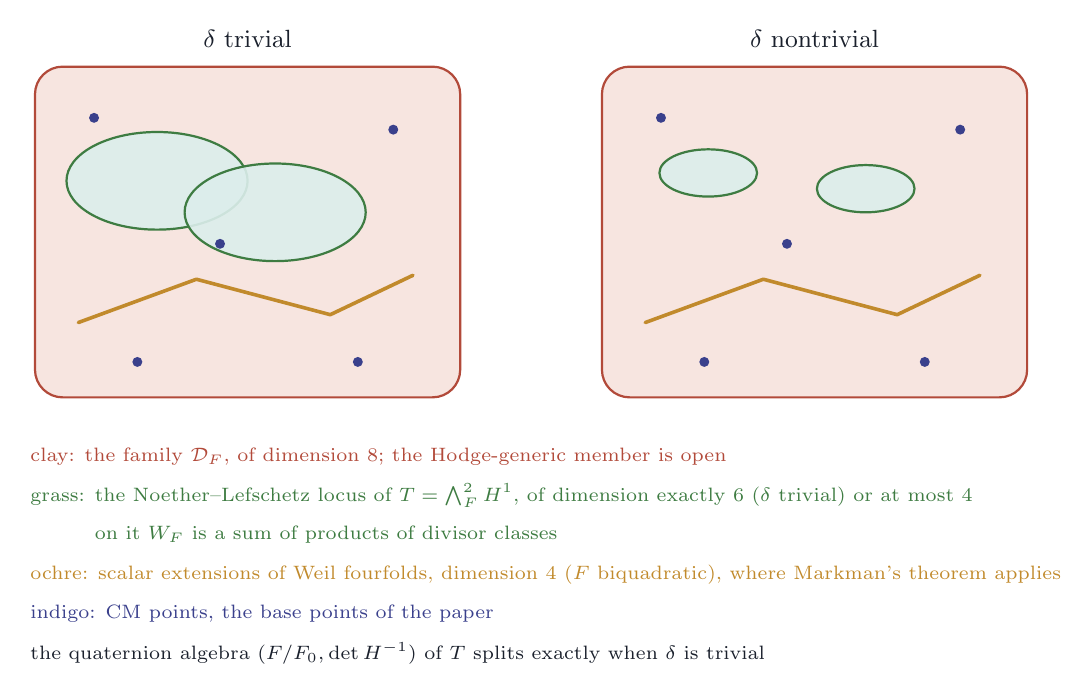
\begin{tikzpicture}[x=1cm,y=1cm,line join=round,line cap=round,
  font=\small,text=PInk]
  \fill[WClay,rounded corners=10pt] (0.00,0.00) rectangle (5.40,4.20);
  \draw[PClay,line width=0.8pt,rounded corners=10pt] (0.00,0.00) rectangle (5.40,4.20);
  \node[text=PInk,inner sep=1pt,align=center,font=\small] at (2.70,4.55) {$\delta$ trivial};
  \fill[WTeal,opacity=0.9] (1.55,2.75) ellipse (1.15 and 0.62);
  \draw[PGrass,line width=0.8pt] (1.55,2.75) ellipse (1.15 and 0.62);
  \fill[WTeal,opacity=0.9] (3.05,2.35) ellipse (1.15 and 0.62);
  \draw[PGrass,line width=0.8pt] (3.05,2.35) ellipse (1.15 and 0.62);
  \draw[POchre,line width=1.30pt] (0.55,0.95) -- (2.05,1.50) -- (3.75,1.05) -- (4.80,1.55);
  \fill[PIndigo] (0.75,3.55) circle (1.8pt);
  \fill[PIndigo] (2.35,1.95) circle (1.8pt);
  \fill[PIndigo] (4.55,3.40) circle (1.8pt);
  \fill[PIndigo] (4.10,0.45) circle (1.8pt);
  \fill[PIndigo] (1.30,0.45) circle (1.8pt);
  \fill[WClay,rounded corners=10pt] (7.20,0.00) rectangle (12.60,4.20);
  \draw[PClay,line width=0.8pt,rounded corners=10pt] (7.20,0.00) rectangle (12.60,4.20);
  \node[text=PInk,inner sep=1pt,align=center,font=\small] at (9.90,4.55) {$\delta$ nontrivial};
  \fill[WTeal,opacity=0.9] (8.55,2.85) ellipse (0.62 and 0.30);
  \draw[PGrass,line width=0.8pt] (8.55,2.85) ellipse (0.62 and 0.30);
  \fill[WTeal,opacity=0.9] (10.55,2.65) ellipse (0.62 and 0.30);
  \draw[PGrass,line width=0.8pt] (10.55,2.65) ellipse (0.62 and 0.30);
  \draw[POchre,line width=1.30pt] (7.75,0.95) -- (9.25,1.50) -- (10.95,1.05) -- (12.00,1.55);
  \fill[PIndigo] (7.95,3.55) circle (1.8pt);
  \fill[PIndigo] (9.55,1.95) circle (1.8pt);
  \fill[PIndigo] (11.75,3.40) circle (1.8pt);
  \fill[PIndigo] (11.30,0.45) circle (1.8pt);
  \fill[PIndigo] (8.50,0.45) circle (1.8pt);
  \node[text=PClay,inner sep=1pt,align=center,font=\scriptsize,anchor=west] at (-0.10,-0.75) {clay: the family $\cD_{F}$, of dimension $8$; the Hodge-generic member is open};
  \node[text=PGrass,inner sep=1pt,align=center,font=\scriptsize,anchor=west] at (-0.10,-1.25) {grass: the Noether--Lefschetz locus of $T=\bigwedge^{2}_{F}H^{1}$, of dimension exactly $6$ ($\delta$ trivial) or at most $4$};
  \node[text=PGrass,inner sep=1pt,align=center,font=\scriptsize,anchor=west] at (-0.10,-1.75) {\phantom{grass: }on it $W_{F}$ is a sum of products of divisor classes};
  \node[text=POchre,inner sep=1pt,align=center,font=\scriptsize,anchor=west] at (-0.10,-2.25) {ochre: scalar extensions of Weil fourfolds, dimension $4$ ($F$ biquadratic), where Markman's theorem applies};
  \node[text=PIndigo,inner sep=1pt,align=center,font=\scriptsize,anchor=west] at (-0.10,-2.75) {indigo: CM points, the base points of the paper};
  \node[text=PInk,inner sep=1pt,align=center,font=\scriptsize,anchor=west] at (-0.10,-3.25) {the quaternion algebra $(F/F_{0},\det H^{-1})$ of $T$ splits exactly when $\delta$ is trivial};
\end{tikzpicture}
\end{document}
